\chapter{Methodology}

\section{Methodological Approach}

\subsection{Research Paradigm}

This research adopts a pragmatic paradigm \cite{venkatesh2003}, integrating quantitative and qualitative methods to address the complex challenges of hospital medication management. The methodological framework is grounded in Design Science Research (DSR) \cite{martin2017}, which emphasizes the creation and evaluation of innovative artifacts—in this case, an integrated software system—designed to solve real-world problems within a specific organizational context. The DSR approach is particularly well-suited for this project, as it provides a rigorous structure for developing a technologically-sound solution while ensuring its practical relevance and utility in the SCMVV hospital environment.

\subsection{Research Strategy}

The investigation employed an Action Research strategy \cite{greenhalgh2017}. This cyclical and iterative approach involves continuous cycles of planning, acting, observing, and reflecting. It allows for the incremental improvement of the system based on empirical feedback gathered directly from the clinical setting. This strategy was chosen due to the dynamic nature of the hospital environment and the need to adapt the system to the unique workflows and emergent requirements of the SCMVV. By actively involving practitioners in the research process, this strategy fosters co-creation of knowledge and ensures the final artifact is aligned with user needs.

\section{Research Design}

\subsection{Research Questions}

The study was guided by the following primary research questions:

\begin{enumerate}
    \item How can an integrated medication management system effectively reduce medication errors and enhance patient safety in a hospital setting?
    \item What are the critical success factors for the design, implementation, and adoption of a new medication management system within a complex clinical workflow?
    \item How can the effectiveness of a medication management system be rigorously evaluated in terms of its impact on patient safety, operational efficiency, and user satisfaction?
\end{enumerate}

\subsection{Research Objectives}

The main objective of this research is to develop and evaluate an integrated medication management system that enhances patient safety and improves the efficiency of clinical processes at the SCMVV.

This overarching goal is broken down into the following specific objectives:
\begin{enumerate}
    \item To conduct a thorough analysis of the existing medication management processes at SCMVV to identify critical failure points and opportunities for improvement.
    \item To design and develop an evidence-based, integrated system that addresses the identified gaps and leverages modern software engineering principles.
    \item To implement the system in a controlled, real-world hospital environment, ensuring minimal disruption to ongoing clinical activities.
    \item To systematically evaluate the impact of the system on key performance indicators related to patient safety, operational efficiency, and user acceptance.
\end{enumerate}

\section{Development Methodology}

\subsection{Development Model}

The system was developed using an adapted agile methodology \cite{fowler2018}, which blends principles from user-centered design and rapid prototyping. This hybrid approach was selected to facilitate continuous engagement with healthcare professionals and maintain the flexibility needed to respond to evolving requirements throughout the development lifecycle. It emphasizes iterative development, frequent feedback loops, and collaborative problem-solving, ensuring the final product is both robust and clinically relevant.

\subsection{Investigation Phases}

\begin{figure}[htbp]
    \centering
    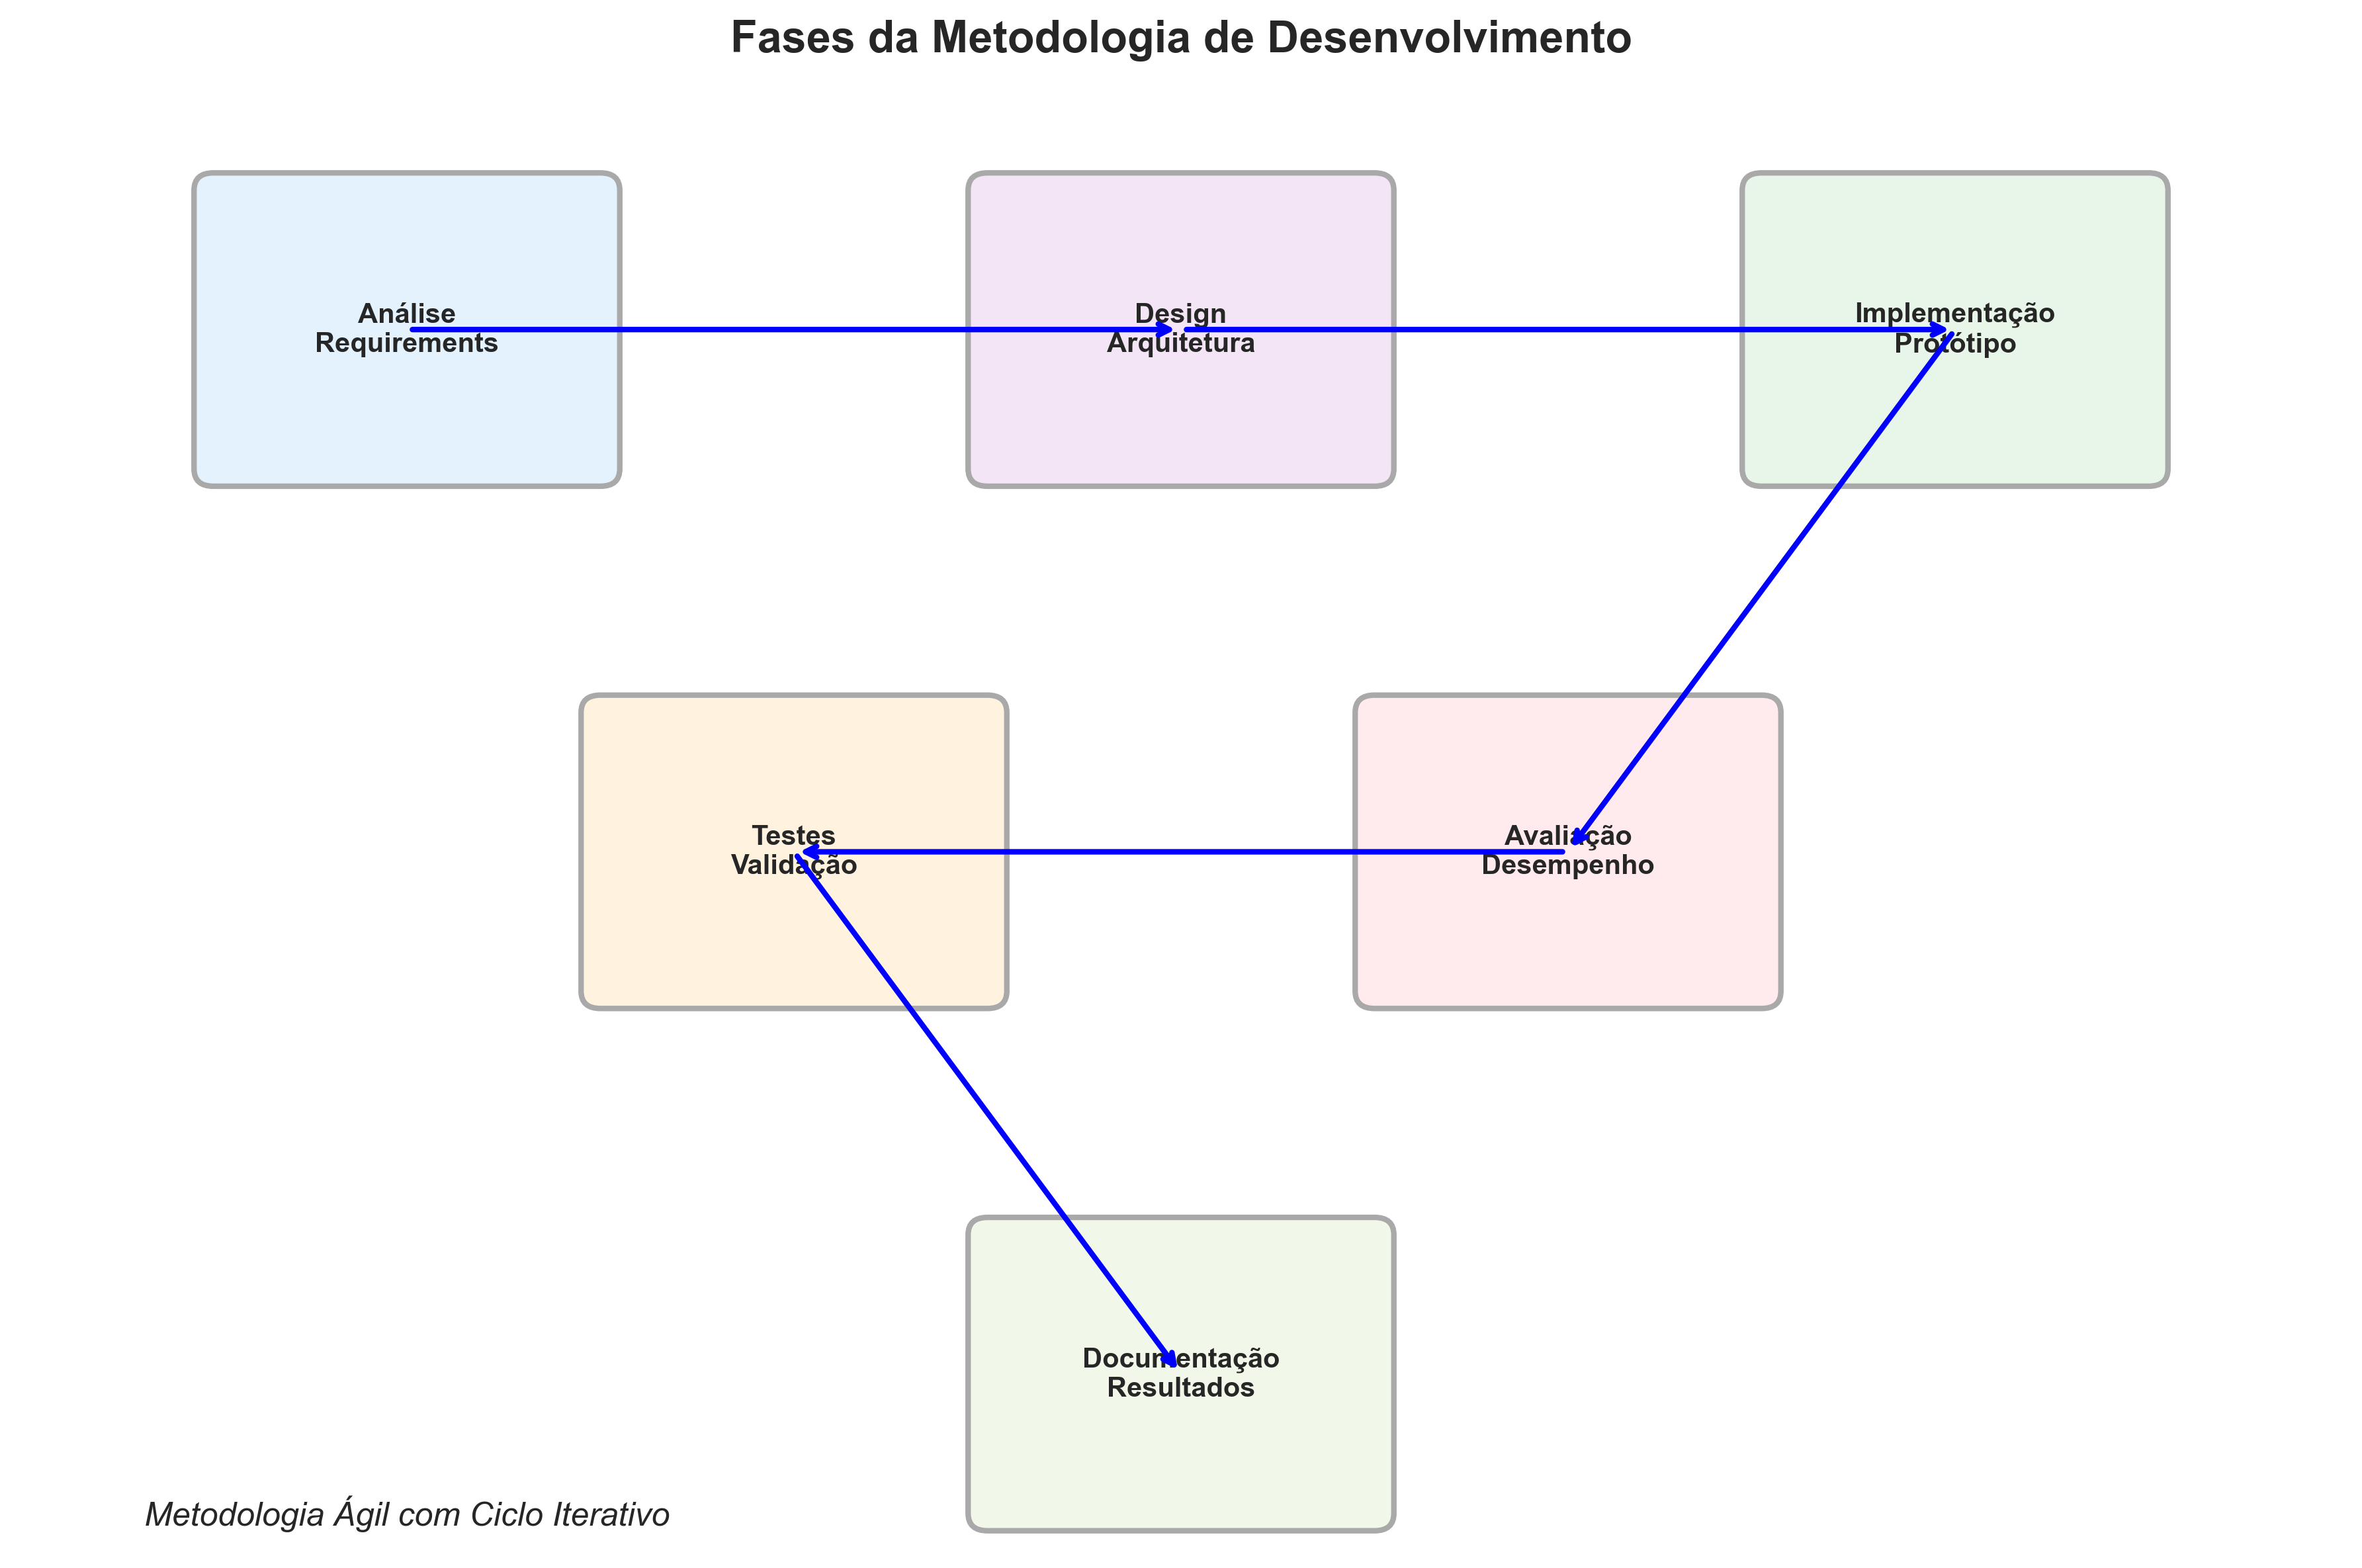
\includegraphics[width=0.9\textwidth]{images/generated/methodology_phases.png}
    \caption{Phases of the research and development methodology for the medication management system.}
    \label{fig:methodology_phases}
\end{figure}

\textbf{Phase 1: Analysis and Diagnosis}
- Systematic literature review.
- In-depth analysis of current workflows at SCMVV.
- Elicitation and documentation of functional and non-functional requirements.

\textbf{Phase 2: Design and Prototyping}
- Development of low-fidelity and high-fidelity functional prototypes.
- Validation sessions with healthcare professionals (physicians, nurses, pharmacists).
- Iterative refinement of requirements and user interface design.

\textbf{Phase 3: Implementation and Testing}
- Development of the final, production-ready system.
- Rigorous unit, integration, and usability testing.
- Validation in a controlled pre-production environment.

\textbf{Phase 4: Evaluation and Validation}
- Pilot implementation in a selected department at SCMVV.
- Collection of quantitative and qualitative performance data.
- Comprehensive analysis of results and system impact.

\section{Data Collection Methods}

\subsection{Quantitative Data}

\textbf{Performance Metrics:}
- System response time and latency.
- Medication error rates (prescribing, dispensing, administration).
- Process efficiency (time spent on prescription, validation, and administration tasks).
- System availability and uptime.

\textbf{Usage Metrics:}
- Number of active users by professional category.
- Feature usage frequency and user navigation patterns.
- Task completion rates and times.

\subsection{Qualitative Data}

\textbf{Semi-Structured Interviews:}
- In-depth interviews with healthcare professionals (physicians, nurses, pharmacists).
- Discussions with hospital managers and IT administrators.

\textbf{Participant Observation:}
- Direct observation of clinical workflows before and after implementation.
- Identification of practical challenges, workarounds, and opportunities.
- Assessment of the system's integration into existing work practices.

\section{Evaluation Criteria}

\subsection{Effectiveness Criteria}

\textbf{Patient Safety:}
- Quantifiable reduction in medication errors \cite{ciapponi2021}.
- Improved traceability of medications from pharmacy to patient.
- Reduction in preventable adverse drug events.

\textbf{Operational Efficiency:}
- Reduction in process cycle times.
- Enhanced interdisciplinary communication and collaboration.
- Optimization of resource utilization (e.g., pharmacist and nurse time).

\subsection{Acceptance Criteria}

\textbf{Usability:}
- System Usability Scale (SUS) scores.
- User satisfaction ratings and qualitative feedback.
- Perceived ease of use and time to proficiency.

\textbf{Adoption:}
- System adoption rates across different professional groups.
- Frequency and depth of feature usage.
- Measurement of resistance to change using established models \cite{venkatesh2003}.

\section{Validation and Verification}

\subsection{Functional Validation}

The system's functionality was validated through:
- A comprehensive suite of automated and manual tests in a staging environment.
- Verification of compliance with all documented clinical and technical requirements.
- End-to-end testing of integration points with legacy systems.

\subsection{Clinical Validation}

\textbf{Pilot Study:}
- Controlled implementation in a specific clinical service.
- Comparison of performance metrics against the baseline established with the legacy system.
- Analysis of the impact on patient safety and workflow quality.

\textbf{Success Criteria:}
- A statistically significant reduction in medication error rates.
- Positive acceptance and feedback from the participating healthcare professionals.
- Measurable improvement in hospital quality indicators.

\section{Ethical Considerations}

\subsection{Data Protection}

This study adhered strictly to the General Data Protection Regulation (GDPR) \cite{european2016}. All patient data was fully anonymized prior to analysis. Informed consent was obtained from all participating healthcare professionals. Robust security measures were implemented to ensure the confidentiality and integrity of all collected information.

\subsection{Ethical Approval}

The research protocol was submitted to and approved by the Ethics Committee of the SCMVV, ensuring compliance with all institutional and national ethical guidelines for research involving health data and human subjects.

\section{Study Limitations}

\subsection{Methodological Limitations}

- The study was conducted at a single hospital, which may limit the generalizability of the findings.
- The post-implementation observation period was limited to six months.
- The absence of a parallel control group constrains the study to a pre-post comparison design.
- A potential for selection bias exists, as volunteers for the pilot may have been more technologically inclined.

\subsection{Technical Limitations}

- The integration with certain external systems was partial due to legacy constraints.
- The system's architecture relies on an existing, centralized Oracle database infrastructure.
- The study operated under defined computational resource constraints.

\section{Execution Timeline}

\begin{figure}[htbp]
    \centering
    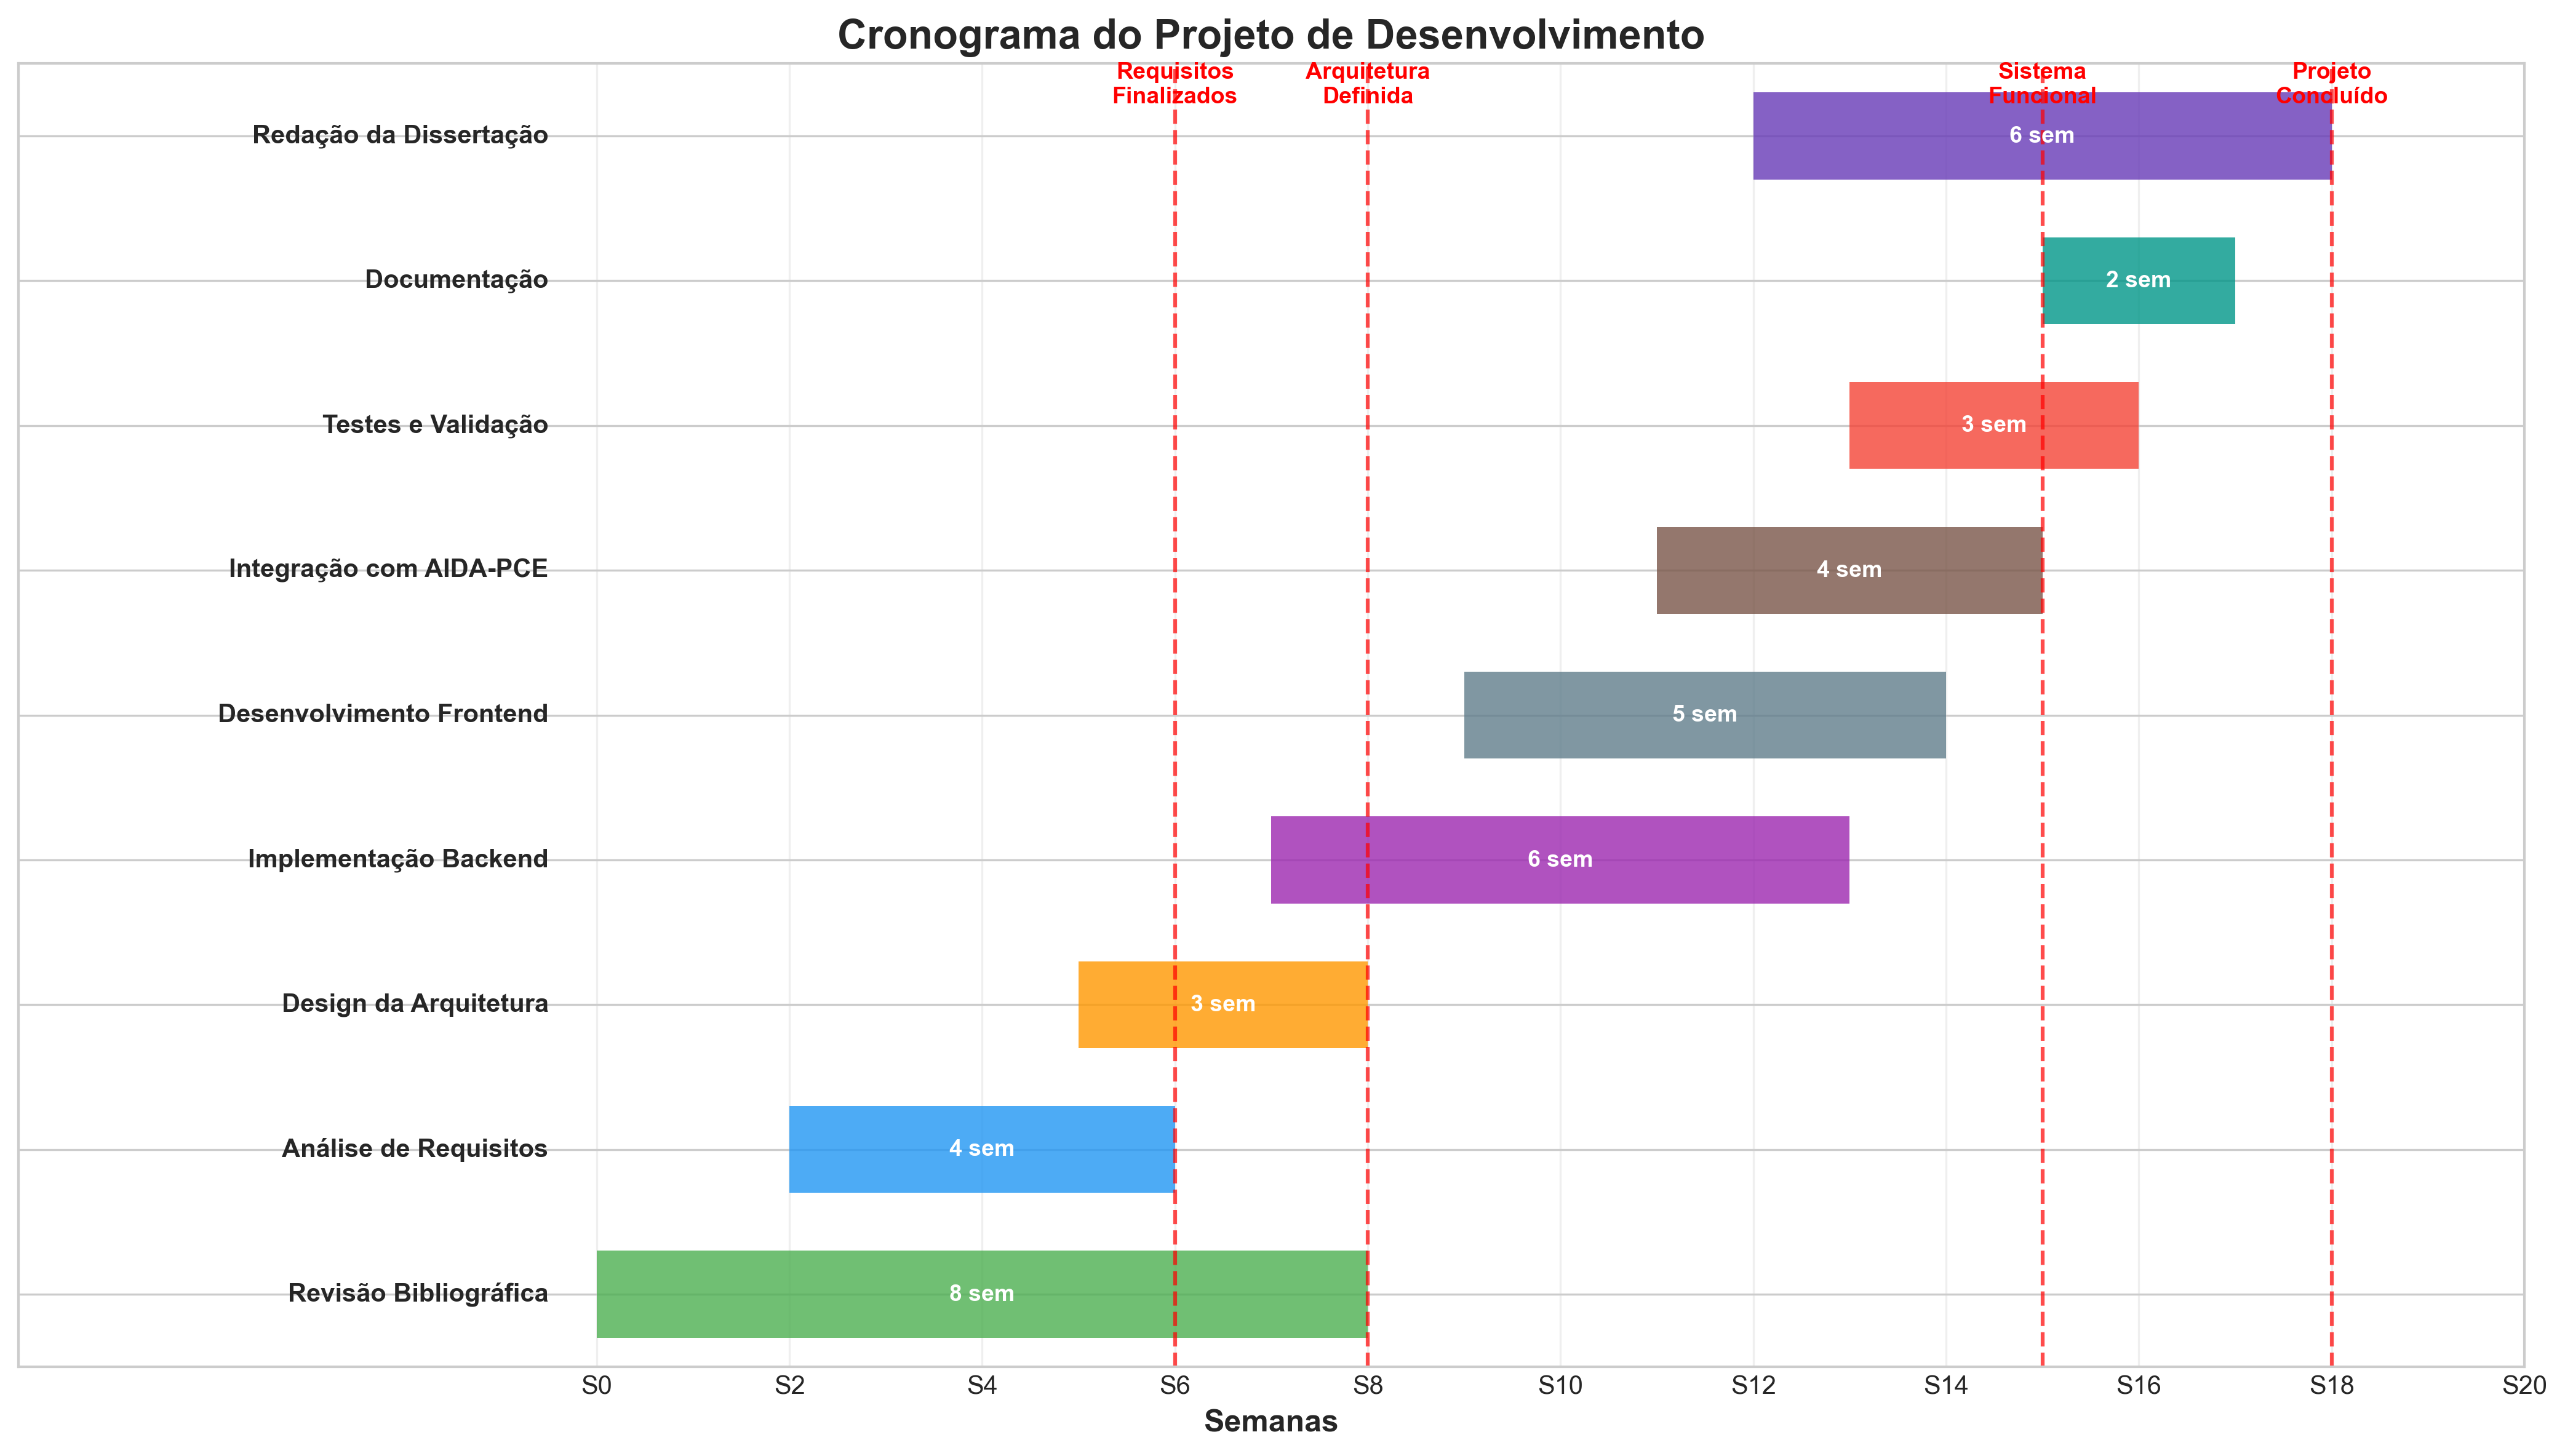
\includegraphics[width=0.95\textwidth]{images/generated/project_timeline.png}
    \caption{Gantt chart illustrating the project's execution timeline, including key phases and milestones.}
    \label{fig:project-timeline}
\end{figure}

The project followed a rigorous 12-month timeline, with well-defined milestones and continuous evaluation points. Each phase included specific objectives, deliverables, and success criteria to ensure structured and measurable progress.